\section{QGIS}
\AtBeginSection[]
{
	\begin{frame}<beamer>
		\frametitle{Plan}
		\tableofcontents[currentsection]
	\end{frame}
}

\begin{frame}{QGIS}
		\begin{block}{Requirement}
			\begin{itemize}
				\item General mapping and analysis
				\item Basic settings and configurations
				\item Print templates
				\item Specific tools and plugins 
				\item Connections to various OGC services
				\item Support and training
			\end{itemize}
		\end{block}
\end{frame}


\subsection{Installer}
\begin{frame}{QGIS installer}

	\centering{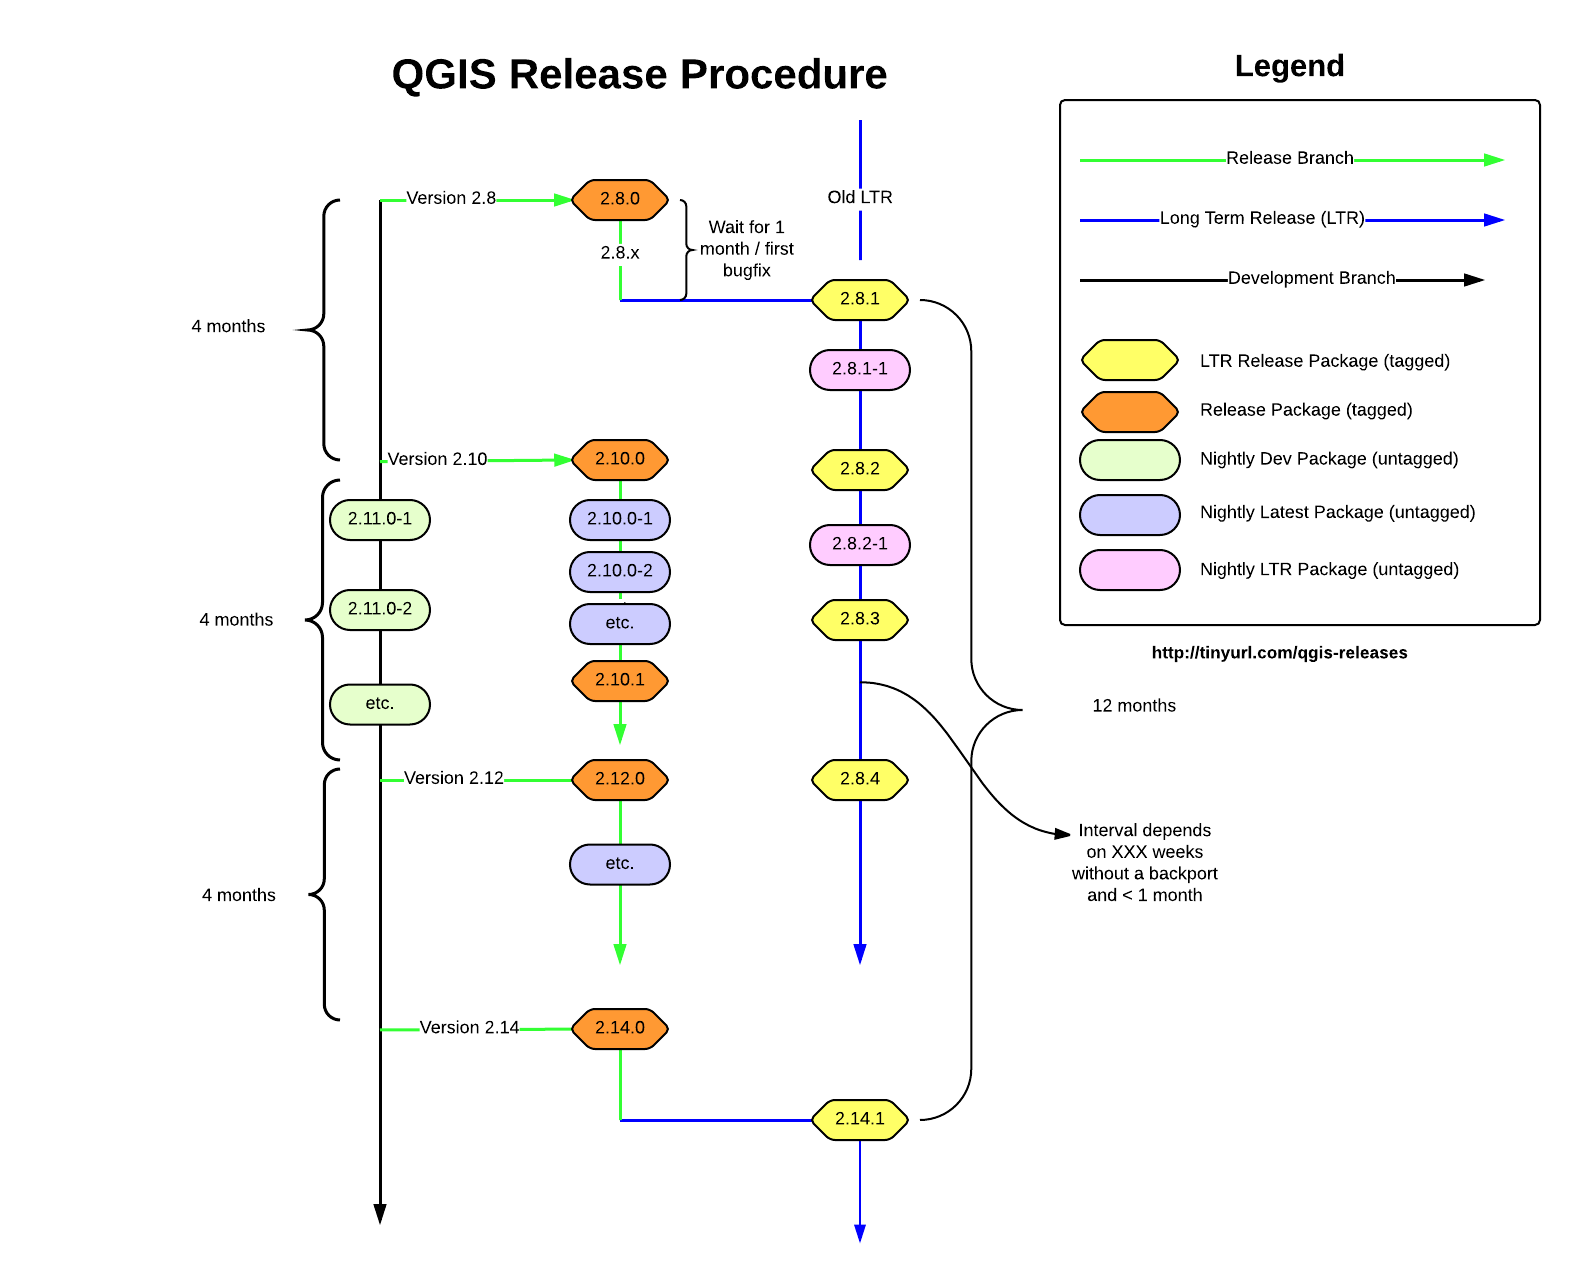
\includegraphics[width=0.9\textwidth]{ae1c0956-523e-11e4-95d9-cea1a3429faf.png}}

\end{frame}


\begin{frame}{QGIS installer}
	
	\centering{\includegraphics[width=0.9\textwidth]{NCCInstaller.png}}
	
\end{frame}

\subsection{Plugins}


\subsection{Settings and configurations}


\subsection{Training}


\subsection{Support}

\section{PostGIS}

\subsection{Migrating data}
\subsection{Sync tool with ArcSDE}

\section{WebGIS and Geoserver}
\subsection{Data preparation}
\subsection{WMS}
\subsection{Internal web map}

